\documentclass[11pt]{article}
\usepackage[T1]{fontenc}
\usepackage[utf8]{inputenc}
\usepackage{lmodern}
\usepackage{microtype}
\usepackage[margin=1in]{geometry}
\usepackage{amsmath,amssymb}
\usepackage{graphicx}
\usepackage{booktabs,longtable,array,calc}
\usepackage{caption}
\captionsetup{font=small,labelfont=bf}
\usepackage{enumitem}
\setlist{itemsep=2pt}
\usepackage{etoolbox}
\usepackage{xurl}
\makeatletter\def\verbatim@font{\fontsize{8}{9.6}\selectfont\ttfamily}\makeatother
\AtBeginEnvironment{longtable}{\small}
\usepackage{xcolor}
\usepackage[colorlinks=true,linkcolor=blue!50!black,urlcolor=blue!50!black,citecolor=blue!50!black]{hyperref}
\usepackage{fancyhdr}
\pagestyle{fancy}
\fancyhf{}
\fancyhead[C]{\small\scshape LDTMP Specification 1.0}
\fancyfoot[C]{\thepage}
\renewcommand{\headrulewidth}{0.4pt}
\setcounter{secnumdepth}{0}
\setlength{\parskip}{4pt}
\setlength{\emergencystretch}{3em}
\setlength{\parindent}{0pt}
\providecommand{\tightlist}{\setlength{\itemsep}{0pt}\setlength{\parskip}{0pt}}

\title{LDTMP: A Layered Depth Tension Modulation Protocol for Pacing
Emotional Depth in AI-Led Conversations}
\author{Alexander
Milovidov\\[2pt]\small Independent researcher\\\small\url{https://github.com/amilovidov/ldtmp}}
\date{Technical report, Specification 1.0, 2026-10-23}

\begin{document}
\maketitle
\thispagestyle{empty}

\begin{abstract}
AI interviewers built on large language models can hold fluent
conversations, yet they have no principled way to decide how personal a
conversation should become or when. Research on sycophancy suggests that
a model left to judge a person's readiness for deeper questions will
tend to agree with the direction the conversation already has (Section
2.4). This report specifies LDTMP, a protocol that moves that decision
out of the model. LDTMP defines six conversation layers that deepen from
rapport to the most personal material and then lighten toward a
forward-looking close. Deterministic rules move a session between layers
using behavioral signals computed from each response: length, latency,
vocabulary diversity, emotional expression and trends across the
session. A safety gate can veto any move into a deeper layer. The model
writes one question at a time inside constraints set by the current
layer. The report gives the full rule set and its constants, proves that
the safety gate can bind only at the icebreaker's exchange cap, and
works three examples through the formulas. It also documents three
defects found in the first production implementation and the tests that
catch them. An internal benchmark of that implementation was
inconclusive, so LDTMP remains unevaluated, and its thresholds are
hand-tuned starting values.

\medskip
\noindent\textbf{Keywords:} conversational agents, large language models, conversation design,
self-disclosure, engagement signals, AI interviewers
\end{abstract}

\section{1. Introduction}

An interview has a shape. Skilled interviewers open with easy questions,
build rapport, move toward the material that matters, and close in a way
that leaves the other person steady. They also read when the other
person is not ready to go further, and they step back.

Language-model interviewers reproduce the surface of this skill without
its structure. A model prompted to ``go deeper when appropriate''
decides depth implicitly, one turn at a time, with no explicit state and
no record of why it chose. Two failures follow from that design. A model
can push a disengaged person toward heavy topics because the prompt
invited depth, and it can stay at small talk for an entire session
because nothing required it to advance. Neither failure is visible after
the fact, because the decision was never made explicitly.

LDTMP splits the work in two. A deterministic controller holds the
conversation's position in a fixed six-layer arc and moves it only when
measured signals satisfy explicit rules. The language model receives the
current layer's constraints with every request and writes within them.
The protocol was first built for a voice-first app that interviews
people about their memories and turns those conversations into written
stories, and it ran in production in that app.

This report makes four contributions:

\begin{enumerate}
\def\labelenumi{\arabic{enumi}.}
\tightlist
\item
  A specification, detailed enough to implement, of the six layers,
  their generation constraints, the signal formulas, the transition
  rules and the safety gate, with every constant published in
  machine-readable form.
\item
  A short analysis of the protocol's properties. It proves that, when
  signals are derived as specified, the safety gate can bind in only one
  situation, and Example B shows that it does.
\item
  Three worked examples, computed from the formulas, that
  implementations can check their arithmetic against.
\item
  A record of three defects from the first production implementation and
  the tests that catch them.
\end{enumerate}

\subsection{1.1 Scope and non-clinical status}

LDTMP is a conversation-design protocol. I have not validated it as
therapy or as a clinical intervention, and it makes no claim to be
either. Several of the cited sources come from counseling research, and
LDTMP borrows only their approach to pacing.

The safety score in this specification is a pacing control. It keeps the
system from pushing a disengaged person toward heavier topics. It does
not detect crisis, self-harm risk or distress, and an implementation
must not present it as doing so. Any product that may meet people in
distress needs a separate, purpose-built escalation path.

\subsection{1.2 Conventions}

The key words MUST, MUST NOT, SHOULD and MAY follow RFC 2119. Every
numeric constant in this report, including the transition rules of Table
4, also appears in \href{ldtmp.config.json}{\texttt{ldtmp.config.json}},
and an agent implementing the protocol SHOULD load every number from
that file. Times are in milliseconds unless a unit is stated. Scores are
real numbers clamped to the closed interval {[}0, 1{]}.

\section{2. Background and related work}

\subsection{2.1 Graduated self-disclosure}

Social penetration theory describes relationships as deepening through a
gradual increase in the breadth and depth of what people disclose to
each other (Altman \& Taylor, 1973). Disclosure proceeds in layers, from
public facts toward private values and feelings. Aron et al.~(1997)
turned the idea into a procedure. Pairs of strangers who took turns
answering questions that escalated in personal depth over 45 minutes
reported greater closeness than pairs who held small talk for the same
time. LDTMP adopts the premise that depth should increase in a fixed
order. It also adds explicit conditions for advancing and for
retreating. Its interviewer does not disclose in return, so it drops the
reciprocity of the original procedure.

\subsection{2.2 Pacing in narrative and motivational practice}

Narrative practice treats the stories people tell about their lives as
open to re-authoring, and it attends to experiences that the dominant
story leaves out (White \& Epston, 1990). Motivational interviewing
describes a guiding style that evokes the person's own reasons and
adjusts to their readiness for change (Miller \& Rollnick, 2013). LDTMP
takes from both traditions the practice of building each question on
what the person has just said. Their clinical aims are out of scope.
LDTMP's climb back from the peak through a relief layer to a
forward-looking close rests on a design premise of mine, that a
conversation which reaches difficult material should not end there.

\subsection{2.3 Behavioral signals of engagement}

Listeners use response latency and filled pauses to judge whether a
speaker knows the answer to a question, and a long delay before an
answer lowers that judgment (Brennan \& Williams, 1995). That finding
motivates LDTMP's use of latency as a signal, though it concerns
knowledge and the protocol uses latency for engagement. Speakers also
use ``uh'' and ``um'' to announce a minor or a major delay in speaking
(Clark \& Fox Tree, 2002). Filler counts and the timing of turns (Sacks
et al., 1974) are natural inputs for the voice extension described in
Section 6.4.

The protocol's other measures, such as word counts, unique-word ratios,
emotion-marker counts and trend flags across the session, are
engineering heuristics of mine. No cited study validated them, and
Section 6.2 treats the gap as a limitation.

\subsection{2.4 Agreement bias in language models}

Language models trained with human feedback show sycophancy, a tendency
to tell users what they appear to want to hear. Human preference
judgments themselves favor such responses some of the time (Sharma et
al., 2023). The bias matters for depth control. A model asked whether a
person is ready for a more personal question receives a prompt that
already frames depth as the goal. I expect agreement to be the likely
answer, though Sharma et al.~did not test this kind of judgment, so the
risk is an extrapolation. LDTMP takes that judgment away from the model.
A model may still help measure the signals, for example by counting
emotional statements, but it never decides the layer. This is the
protocol's central design choice.

\section{3. The protocol}

\subsection{3.1 Design principles}

\textbf{P1. Deterministic layer decisions.} The layer decision is a pure
function of measured signals and session state. It runs before
generation, and its output becomes part of the prompt.

\textbf{P2. Layers constrain by explicit lists.} Each layer lists
recommended topics, topics to avoid, a word range for the question and
an emotional intensity. Those boundaries leave the model free to respond
to what the person said.

\textbf{P3. Asymmetric transitions.} Moving deeper requires time in the
current layer, sustained engagement and evidence of depth, and it can
only advance one layer at a time. Moving back toward a lighter layer
needs only a disengagement signal and a weak answer, and each retreat
steps back one layer. After the peak, disengagement moves the session
toward the close and never back into heavier material.

\textbf{P4. Every decision carries its reasons.} The layer decision
returns the inputs it used, the rule that fired and a confidence value.
That record lets a person audit a session after the fact, and it gives
an evaluation harness something to assert against.

\subsection{3.2 The six layers}

The layers form an arc that rises and comes back down. The sequence
order in Table 1 is the order of progression. The intensity column gives
the emotional weight of questions in each layer, and it falls again
after the peak.

\begin{longtable}[]{@{}
  >{\raggedright\arraybackslash}p{(\linewidth - 6\tabcolsep) * \real{0.1020}}
  >{\raggedright\arraybackslash}p{(\linewidth - 6\tabcolsep) * \real{0.3776}}
  >{\raggedright\arraybackslash}p{(\linewidth - 6\tabcolsep) * \real{0.1531}}
  >{\raggedright\arraybackslash}p{(\linewidth - 6\tabcolsep) * \real{0.3673}}@{}}
\caption{The six conversation layers in order of progression, with the
emotional intensity of each.}\tabularnewline
\toprule\noalign{}
\begin{minipage}[b]{\linewidth}\raggedright
\#
\end{minipage} & \begin{minipage}[b]{\linewidth}\raggedright
Layer
\end{minipage} & \begin{minipage}[b]{\linewidth}\raggedright
Intensity
\end{minipage} & \begin{minipage}[b]{\linewidth}\raggedright
Purpose
\end{minipage} \\
\midrule\noalign{}
\endfirsthead
\toprule\noalign{}
\begin{minipage}[b]{\linewidth}\raggedright
\#
\end{minipage} & \begin{minipage}[b]{\linewidth}\raggedright
Layer
\end{minipage} & \begin{minipage}[b]{\linewidth}\raggedright
Intensity
\end{minipage} & \begin{minipage}[b]{\linewidth}\raggedright
Purpose
\end{minipage} \\
\midrule\noalign{}
\endhead
\bottomrule\noalign{}
\endlastfoot
0 & \texttt{ICEBREAKER} & light & Build rapport and lower the cost of
answering. \\
1 & \texttt{SURFACE} & light & Open the topic with broad, easy
questions. \\
2 & \texttt{INITIAL\_\allowbreak{}DESCENT} & moderate & Ask what the experience meant
and how it felt. \\
3 & \texttt{EMOTIONAL\_\allowbreak{}SATURATION} & deep & Stay present with the
strongest material the person chooses to share. \\
4 & \texttt{RELIEF\_\allowbreak{}ARC} & moderate & Turn toward perspective, strength
and what was learned. \\
5 & \texttt{REENTRY} & light & Close the conversation and look
forward. \\
\end{longtable}

The ``tension modulation'' in the protocol's name refers to this shape.
Tension rises through layers 0 to 3 and resolves through layers 4 and 5.
The rules are built so that the arc resolves. After the peak, no rule
leads back into heavier material, because a conversation that stops at
layer 3 leaves the person at the heaviest point of the session. Section
4.3 shows that a session can still stay at the peak.

Figure 1 shows the arc as a state machine. Forward moves advance one
layer at a time, and the safety gate covers the three moves before the
peak. Each retreat rule in Table 4 steps back one layer, and only the
three layers up to the peak have one.

\begin{figure}[t]
\centering
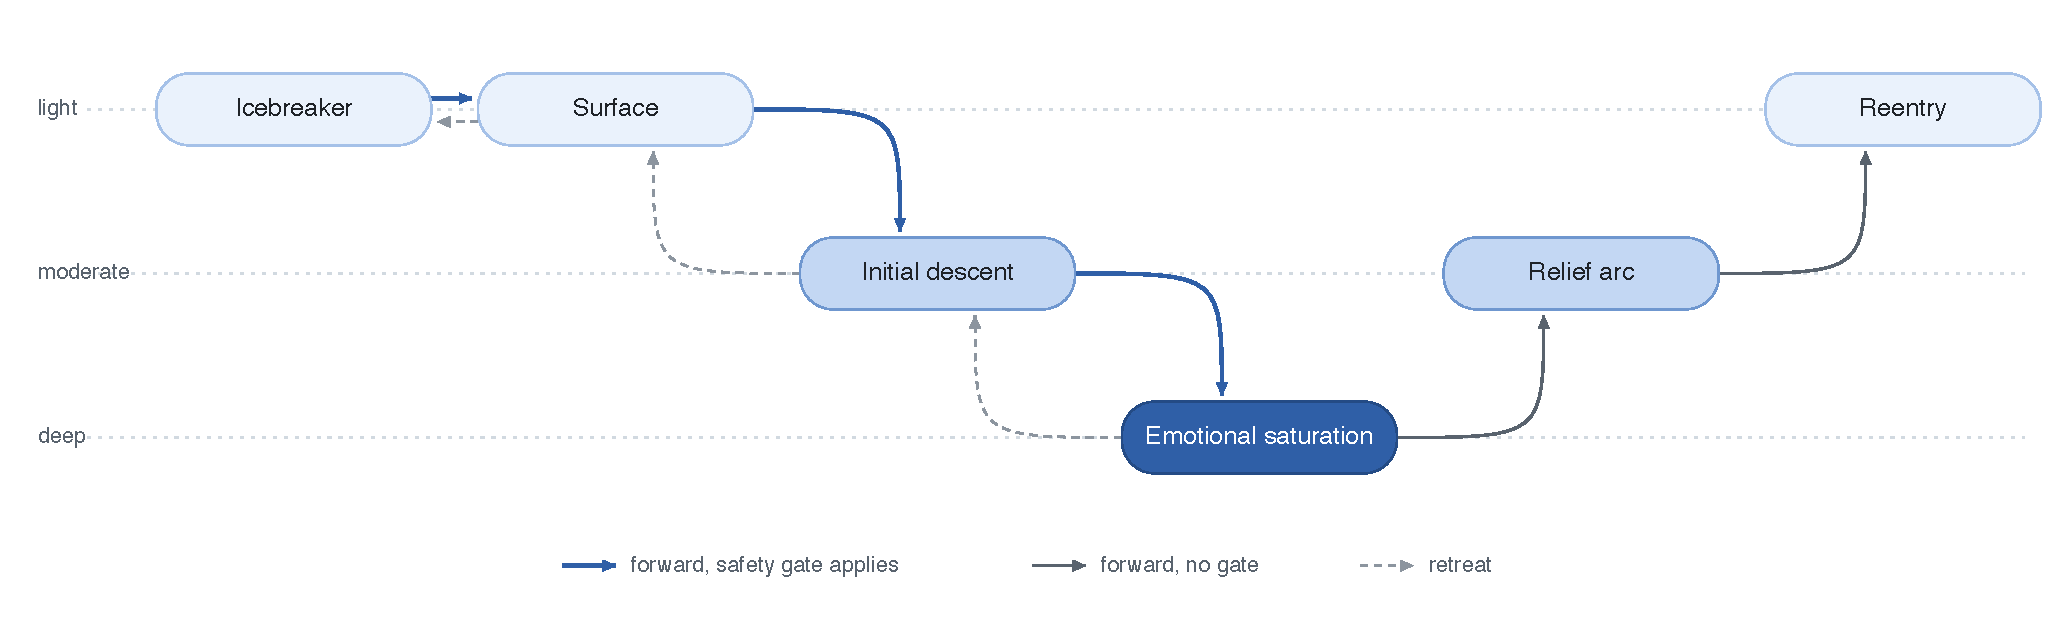
\includegraphics[width=\linewidth]{fig1-layer-arc.pdf}
\caption{The six layers placed by emotional intensity, so the descent to the peak and the climb back out are visible. Thick blue arrows are forward moves that the safety gate covers, thin gray arrows are ungated forward moves, and dashed arrows are retreats.}
\label{fig:arc}
\end{figure}

\subsection{3.3 Generation constraints per layer}

The orchestrator passes the constraints in Table 2 to the model with
every generation request. The word range applies to the generated
question. Table 2 abridges the topic lists, and the configuration file
holds them in full.

\begin{longtable}[]{@{}
  >{\raggedright\arraybackslash}p{(\linewidth - 8\tabcolsep) * \real{0.2327}}
  >{\raggedright\arraybackslash}p{(\linewidth - 8\tabcolsep) * \real{0.0881}}
  >{\raggedright\arraybackslash}p{(\linewidth - 8\tabcolsep) * \real{0.2264}}
  >{\raggedright\arraybackslash}p{(\linewidth - 8\tabcolsep) * \real{0.2264}}
  >{\raggedright\arraybackslash}p{(\linewidth - 8\tabcolsep) * \real{0.2264}}@{}}
\caption{Generation constraints that the orchestrator passes to the
model for each layer.}\tabularnewline
\toprule\noalign{}
\begin{minipage}[b]{\linewidth}\raggedright
Layer
\end{minipage} & \begin{minipage}[b]{\linewidth}\raggedright
Question words
\end{minipage} & \begin{minipage}[b]{\linewidth}\raggedright
Recommended topics
\end{minipage} & \begin{minipage}[b]{\linewidth}\raggedright
Topics to avoid
\end{minipage} & \begin{minipage}[b]{\linewidth}\raggedright
Tone
\end{minipage} \\
\midrule\noalign{}
\endfirsthead
\toprule\noalign{}
\begin{minipage}[b]{\linewidth}\raggedright
Layer
\end{minipage} & \begin{minipage}[b]{\linewidth}\raggedright
Question words
\end{minipage} & \begin{minipage}[b]{\linewidth}\raggedright
Recommended topics
\end{minipage} & \begin{minipage}[b]{\linewidth}\raggedright
Topics to avoid
\end{minipage} & \begin{minipage}[b]{\linewidth}\raggedright
Tone
\end{minipage} \\
\midrule\noalign{}
\endhead
\bottomrule\noalign{}
\endlastfoot
\texttt{ICEBREAKER} & 8 to 20 & the current moment, simple facts, light
preferences, recent activities & trauma, loss, deep relationships,
existential questions, heavy emotions, vulnerability & A warm greeting
and one natural question, like catching up with a friend. \\
\texttt{SURFACE} & 10 to 25 & daily life, hobbies, interests, work
overview, family basics, recent experiences & trauma, loss, deep fears,
existential crisis, intense emotions & React warmly to the answer, then
ask one curious follow-up. \\
\texttt{INITIAL\_\allowbreak{}DESCENT} & 12 to 20 & meaningful relationships, values,
life choices, challenges faced, growth moments & deep trauma, unresolved
grief, existential dread, severe loss & Thoughtful and concise. One
meaningful question. \\
\texttt{EMOTIONAL\_\allowbreak{}SATURATION} & 18 to 28 & deep emotions, fears,
regrets, turning points, inner conflicts & topics that require
professional help & Deeply attentive. One question. Hold space and do
not interrogate. \\
\texttt{RELIEF\_\allowbreak{}ARC} & 12 to 20 & resilience, lessons learned, strength
discovered, perspective gained & reopening fresh wounds, minimizing
pain, forced positivity & Supportive and balanced. Acknowledge the
difficulty without minimizing it. \\
\texttt{REENTRY} & 10 to 18 & future outlook, next steps, integration,
grounding & deep emotional topics, unresolved issues, heavy subjects &
Warm and grounding. One forward-looking question. \\
\end{longtable}

Every layer shares these generation rules, and the implementation MUST
include them in the prompt. The model asks exactly one open-ended
question and builds it on a specific detail from the person's last
answer where it can. It avoids clinical or therapeutic vocabulary, and
it never asks again about an emotion the person has already named.

An implementation SHOULD validate each generated question against its
layer. Checking word count and matching keywords against the avoid list
is enough for a first version, and a failed check triggers one
regeneration.

\subsection{3.4 Signals}

LDTMP computes its signals from three sources: the latest response, the
rolling history of responses, and elapsed time. A text-only
implementation can compute all of them. In a text interface, latency
runs from showing the question to receiving the answer, and the stage
directions of Section 3.4.5 count as zero. A voice implementation can
add prosody, though no rule in this specification depends on it.

\subsubsection{3.4.1 Per-response measurements}

For each user response the implementation records the word count, the
latency in seconds between the end of the question and the start of the
answer, the number of unique words, and a count of emotional statements.
An emotional statement is a sentence that expresses a feeling, fear,
aspiration or value. An LLM extraction pass can produce that count in
any language, and a keyword list is an acceptable fallback. The
implementation keeps a rolling history of the last 20 responses in the
session.

\subsubsection{3.4.2 Engagement score}

The engagement score is a composite over the rolling history.

\begin{verbatim}
score = 0.2                                       # base
      + length_points(avg_words)                  # 0.30 if >= 50, 0.20 if >= 30, 0.10 if >= 15, else 0
      + latency_points(avg_latency_s)             # 0.20 if <= 5, 0.15 if <= 15, 0.10 if <= 30, else 0
      + 0.2 * min(avg_unique_words / 20, 1)       # vocabulary diversity
      + 0.1 * min(avg_emotional_statements / 3, 1)
      - 0.20 if decreasing_length
      - 0.15 if increasing_latency
      - 0.40 if straight_line_responding
score = clamp(score, 0, 1)
\end{verbatim}

The three trend flags need at least four responses in the history.
Before that point they are false.

\begin{itemize}
\tightlist
\item
  \texttt{decreasing\_\allowbreak{}length}: the mean word count of the second half of
  the history is below 0.7 times the mean of the first half.
\item
  \texttt{increasing\_\allowbreak{}latency}: the mean latency of the second half
  exceeds 1.5 times the mean of the first half.
\item
  \texttt{straight\_\allowbreak{}line\_\allowbreak{}responding}: each of the last three responses
  has 5 words or fewer.
\end{itemize}

\subsubsection{3.4.3 Engagement level}

The engagement level is an ordinal scale (Table 3). Implementations MUST
compare levels by rank and MUST NOT compare their string labels (see
Section 6.1).

\begin{longtable}[]{@{}
  >{\raggedright\arraybackslash}p{(\linewidth - 4\tabcolsep) * \real{0.1205}}
  >{\raggedright\arraybackslash}p{(\linewidth - 4\tabcolsep) * \real{0.3494}}
  >{\raggedright\arraybackslash}p{(\linewidth - 4\tabcolsep) * \real{0.5301}}@{}}
\caption{Engagement levels with their ordinal ranks and assignment
conditions.}\tabularnewline
\toprule\noalign{}
\begin{minipage}[b]{\linewidth}\raggedright
Rank
\end{minipage} & \begin{minipage}[b]{\linewidth}\raggedright
Level
\end{minipage} & \begin{minipage}[b]{\linewidth}\raggedright
Assigned when
\end{minipage} \\
\midrule\noalign{}
\endfirsthead
\toprule\noalign{}
\begin{minipage}[b]{\linewidth}\raggedright
Rank
\end{minipage} & \begin{minipage}[b]{\linewidth}\raggedright
Level
\end{minipage} & \begin{minipage}[b]{\linewidth}\raggedright
Assigned when
\end{minipage} \\
\midrule\noalign{}
\endhead
\bottomrule\noalign{}
\endlastfoot
0 & \texttt{DISENGAGED} & \texttt{straight\_\allowbreak{}line\_\allowbreak{}responding} is true,
or score $\leq$ 0.2 \\
1 & \texttt{SHOWING\_\allowbreak{}FATIGUE} & \texttt{decreasing\_\allowbreak{}length} and
\texttt{increasing\_\allowbreak{}latency} are both true, or 0.2 \textless{} score $\leq$
0.4 \\
2 & \texttt{MODERATE} & 0.4 \textless{} score $\leq$ 0.6 \\
3 & \texttt{ENGAGED} & 0.6 \textless{} score $\leq$ 0.8 \\
4 & \texttt{HIGHLY\_\allowbreak{}ENGAGED} & score \textgreater{} 0.8 \\
\end{longtable}

The pattern overrides in the first two rows take precedence over the
score bands, and the implementation checks them in the order shown.

\subsubsection{3.4.4 Response quality and topic depth}

These two signals come from the latest response alone.

\textbf{Response quality} is \texttt{minimal} below 10 words,
\texttt{moderate} from 10 to 29 words and \texttt{detailed} at 30 words
or more.

\textbf{Topic depth} is \texttt{deep} when the response has more than 40
words and contains at least one emotional statement. It is
\texttt{moderate} when the response has more than 20 words or contains
an emotional statement. It is \texttt{shallow} otherwise. The flow rules
use a numeric depth score, with \texttt{shallow\ =\ 0.2},
\texttt{moderate\ =\ 0.5} and \texttt{deep\ =\ 0.8}.

\subsubsection{3.4.5 Emotional expression}

Emotional expression scores how much feeling the latest response shows
on its surface. It is a sum of capped components.

\begin{verbatim}
expression = min(0.10 * emotion_marker_words, 0.50)       # words such as "nervous", "grateful", "miss"
           + min(0.15 * emotional_stage_directions, 0.30) # transcript cues such as [laughs], [voice breaking]
           + 0.10 if the response contains an ellipsis
           + min(0.05 * exclamation_marks, 0.15)
expression = min(expression, 1)
\end{verbatim}

The marker list is language-specific, and implementations SHOULD supply
one per supported language. An implementation MAY replace this component
with a model-scored value in {[}0, 1{]}.

\subsubsection{3.4.6 Rhythm and the intervention flag}

The protocol assumes that conversations lose energy in cycles of a few
minutes, an assumption I have not tested. The implementation tracks
minutes since the last intervention, where an intervention is any
deliberate change of approach such as a topic shift, a lighter question
or a short reflection. A \textbf{natural cycle point} occurs at 3
minutes and a \textbf{fatigue cycle point} at 6 minutes.

The \texttt{should\_\allowbreak{}intervene} flag is true when any of these holds:

\begin{itemize}
\tightlist
\item
  \texttt{straight\_\allowbreak{}line\_\allowbreak{}responding} is true
\item
  the engagement score is below 0.4
\item
  \texttt{decreasing\_\allowbreak{}length} and \texttt{increasing\_\allowbreak{}latency} are both
  true
\item
  the session has reached a fatigue cycle point
\item
  the session has reached a natural cycle point and the engagement score
  is below 0.6
\end{itemize}

\subsection{3.5 Readiness and safety scores}

Two derived scores feed the safety gate.

\textbf{Emotional readiness.}

\begin{verbatim}
readiness = 0.4 * engagement_score
          + {detailed: 0.2, moderate: 0.1, minimal: 0}[response_quality]
          + 0.2 * emotional_expression        # Section 3.4.5
          + {deep: 0.2, moderate: 0.1, shallow: 0}[topic_depth]
readiness = clamp(readiness, 0, 1)
\end{verbatim}

\textbf{Safety.}

\begin{verbatim}
safety = 1.0
       - 0.4 if level == DISENGAGED
       - 0.2 if level == SHOWING_FATIGUE
       - 0.3 if straight_line_responding
       - 0.2 if fatigue_trend               # decreasing_length AND increasing_latency
       - 0.2 if readiness < 0.4
       - 0.3 if should_intervene
       + 0.2 if level == HIGHLY_ENGAGED
safety = clamp(safety, 0, 1)
\end{verbatim}

The safety threshold is 0.5. Implementations MAY make it configurable.
Implementations MUST round the safety score to two decimal places before
comparing it with the threshold. Every safety term is a multiple of 0.1,
so rounding is exact, and it stops the order of floating-point
subtraction from moving a score of exactly 0.5 below the threshold.

\subsection{3.6 The layer decision}

The orchestrator calls the layer decision once per user turn, after it
has computed the signals and before it builds the generation prompt.

Figure 2 traces one turn through the protocol. The controller settles
the layer before the model writes anything, and the model's output is
checked against that layer before the person sees it.

\begin{figure}[t]
\centering
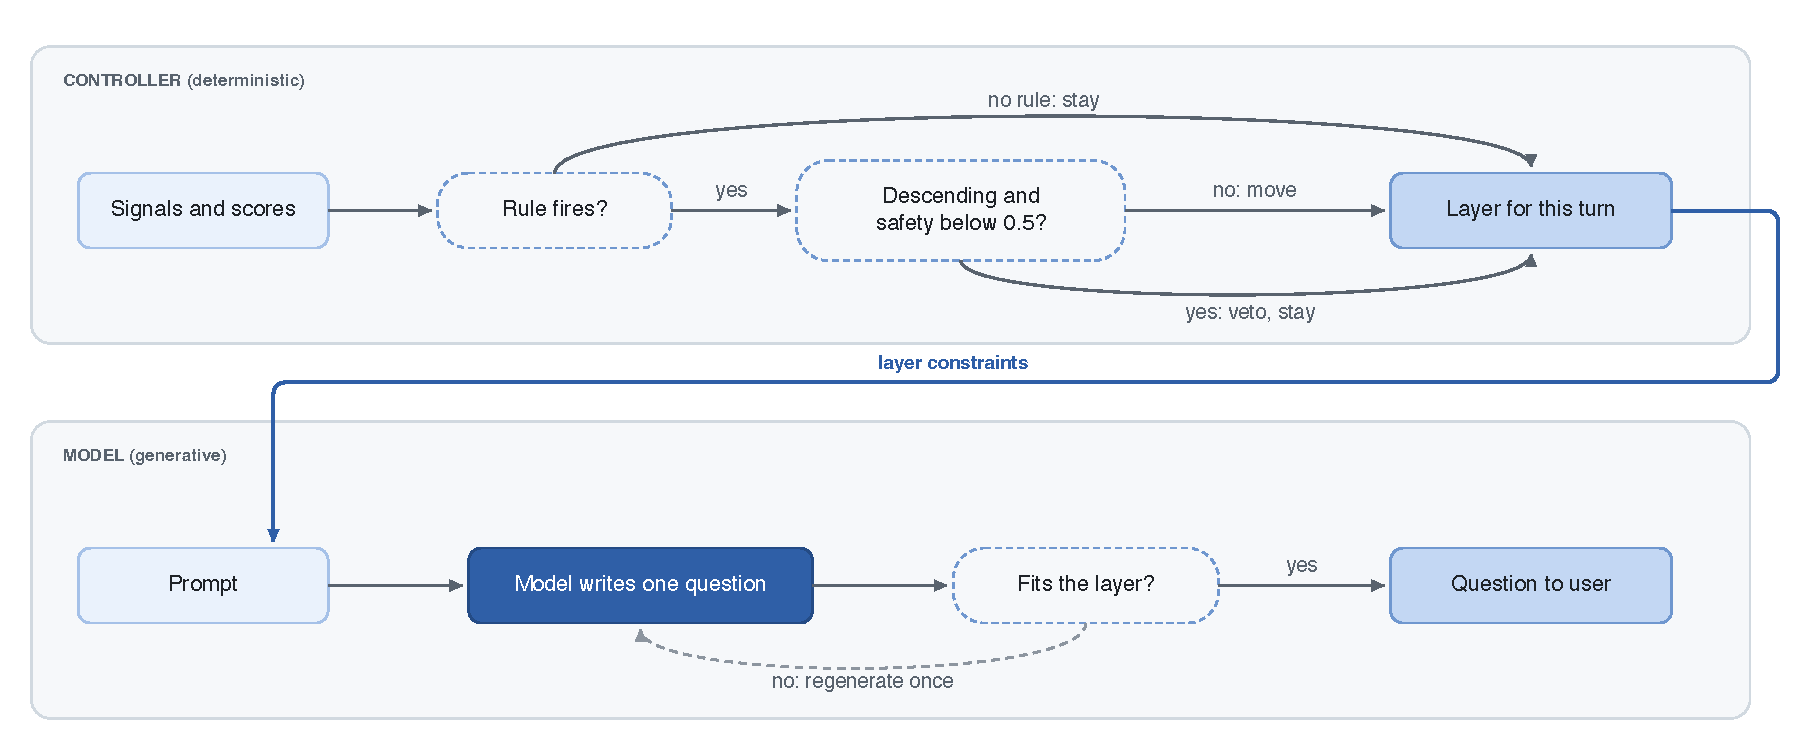
\includegraphics[width=\linewidth]{fig2-one-turn.pdf}
\caption{One turn of the protocol. The deterministic controller settles the layer, and the model then writes and validates a question inside that layer's constraints.}
\label{fig:turn}
\end{figure}

\subsubsection{3.6.1 Session state}

\begin{verbatim}
{
  "current_layer": "ICEBREAKER",
  "exchange_count": 0,        // decisions made so far in this session
  "layer_entered_at": <time>, // reset on every transition
  "session_started_at": <time>
}
\end{verbatim}

Every session starts in \texttt{ICEBREAKER}.

\subsubsection{3.6.2 Transition rules}

The controller evaluates the rules for the current layer in the order
listed in Table 4, and the first match wins. If none match, the session
stays in its current layer. In the table, \texttt{t} is the time spent
in the current layer, \texttt{E} is the engagement level compared by
rank, \texttt{Q} is response quality and \texttt{D} is the numeric depth
score.

\begin{longtable}[]{@{}
  >{\raggedright\arraybackslash}p{(\linewidth - 6\tabcolsep) * \real{0.2913}}
  >{\raggedright\arraybackslash}p{(\linewidth - 6\tabcolsep) * \real{0.2835}}
  >{\raggedright\arraybackslash}p{(\linewidth - 6\tabcolsep) * \real{0.2913}}
  >{\raggedright\arraybackslash}p{(\linewidth - 6\tabcolsep) * \real{0.1339}}@{}}
\caption{Transition rules for each layer, in evaluation order, with the
confidence each rule reports.}\tabularnewline
\toprule\noalign{}
\begin{minipage}[b]{\linewidth}\raggedright
From
\end{minipage} & \begin{minipage}[b]{\linewidth}\raggedright
Rule
\end{minipage} & \begin{minipage}[b]{\linewidth}\raggedright
To
\end{minipage} & \begin{minipage}[b]{\linewidth}\raggedright
Confidence
\end{minipage} \\
\midrule\noalign{}
\endfirsthead
\toprule\noalign{}
\begin{minipage}[b]{\linewidth}\raggedright
From
\end{minipage} & \begin{minipage}[b]{\linewidth}\raggedright
Rule
\end{minipage} & \begin{minipage}[b]{\linewidth}\raggedright
To
\end{minipage} & \begin{minipage}[b]{\linewidth}\raggedright
Confidence
\end{minipage} \\
\midrule\noalign{}
\endhead
\bottomrule\noalign{}
\endlastfoot
\texttt{ICEBREAKER} & \texttt{exchange\_\allowbreak{}count\ $\geq$\ 2} (exchange cap) &
\texttt{SURFACE} & 1.00 \\
\texttt{ICEBREAKER} & \texttt{E\ =\ HIGHLY\_\allowbreak{}ENGAGED} and
\texttt{Q\ =\ detailed} (fast track) & \texttt{SURFACE} & 0.95 \\
\texttt{ICEBREAKER} & \texttt{exchange\_\allowbreak{}count\ $\geq$\ 1} and
\texttt{E\ $\geq$\ MODERATE} & \texttt{SURFACE} & 0.85 \\
\texttt{ICEBREAKER} & no match: stay & & 0.80 \\
\texttt{SURFACE} & \texttt{t\ \textgreater{}\ 60\ s} and
\texttt{E\ $\geq$\ MODERATE} and \texttt{D\ $\geq$\ 0.3} &
\texttt{INITIAL\_\allowbreak{}DESCENT} & 0.80 \\
\texttt{SURFACE} & \texttt{E\ =\ DISENGAGED} and \texttt{Q\ =\ minimal}
& \texttt{ICEBREAKER} & 0.70 \\
\texttt{SURFACE} & no match: stay & & 0.75 \\
\texttt{INITIAL\_\allowbreak{}DESCENT} & \texttt{t\ \textgreater{}\ 120\ s} and
\texttt{E\ =\ HIGHLY\_\allowbreak{}ENGAGED} and \texttt{D\ $\geq$\ 0.6} &
\texttt{EMOTIONAL\_\allowbreak{}SATURATION} & 0.85 \\
\texttt{INITIAL\_\allowbreak{}DESCENT} & \texttt{E\ =\ DISENGAGED} and
\texttt{Q\ =\ minimal} & \texttt{SURFACE} & 0.75 \\
\texttt{INITIAL\_\allowbreak{}DESCENT} & no match: stay & & 0.80 \\
\texttt{EMOTIONAL\_\allowbreak{}SATURATION} & \texttt{t\ \textgreater{}\ 180\ s} and
\texttt{E\ =\ HIGHLY\_\allowbreak{}ENGAGED} and \texttt{D\ $\geq$\ 0.8} &
\texttt{RELIEF\_\allowbreak{}ARC} & 0.90 \\
\texttt{EMOTIONAL\_\allowbreak{}SATURATION} & \texttt{E\ $\leq$\ MODERATE} and
(\texttt{Q\ =\ minimal} or \texttt{D\ \textless{}\ 0.3}) &
\texttt{INITIAL\_\allowbreak{}DESCENT} & 0.80 \\
\texttt{EMOTIONAL\_\allowbreak{}SATURATION} & no match: stay & & 0.85 \\
\texttt{RELIEF\_\allowbreak{}ARC} & \texttt{t\ \textgreater{}\ 60\ s} and
\texttt{E\ $\geq$\ MODERATE} & \texttt{REENTRY} & 0.85 \\
\texttt{RELIEF\_\allowbreak{}ARC} & \texttt{E\ =\ DISENGAGED} and
\texttt{Q\ =\ minimal} & \texttt{REENTRY} & 0.75 \\
\texttt{RELIEF\_\allowbreak{}ARC} & no match: stay & & 0.80 \\
\texttt{REENTRY} & \texttt{E\ =\ DISENGAGED} and \texttt{Q\ =\ minimal}:
stay and offer to end the session & & 0.80 \\
\texttt{REENTRY} & no match: stay & & 0.95 \\
\end{longtable}

Every transition in Table 4 moves exactly one layer, forward or back.
After the peak, the session moves only toward \texttt{REENTRY}. Because
\texttt{exchange\_\allowbreak{}count} is session-wide, a session that retreats to
\texttt{ICEBREAKER} meets the exchange cap at once, and only the safety
gate can hold it there.

\subsubsection{3.6.3 The safety gate}

The safety gate applies to every \textbf{descending} transition. A
descending transition moves deeper into the arc. A descending transition
is any forward move before the peak, so its target is \texttt{SURFACE},
\texttt{INITIAL\_\allowbreak{}DESCENT} or \texttt{EMOTIONAL\_\allowbreak{}SATURATION}. The move
into \texttt{SURFACE} keeps the same light intensity, and the gate
covers it because leaving the icebreaker before the person has warmed up
at all wastes the rapport phase. When the safety score is below the
threshold, the gate vetoes the transition, the session stays in its
current layer, and the decision reports confidence 0.90.

The gate MUST NOT apply to moves into \texttt{RELIEF\_\allowbreak{}ARC} or
\texttt{REENTRY}. Those moves come after the peak and reduce intensity,
and blocking them would hold a struggling person at the heaviest point
of the conversation. The gate also never applies to backward
transitions.

The gate overrides the \texttt{ICEBREAKER} exchange cap. A person who is
disengaged at the cap stays in \texttt{ICEBREAKER}, and the orchestrator
should treat that as a signal to change approach or offer to end the
session.

\subsubsection{3.6.4 Decision output}

\begin{verbatim}
{
  "target_layer": "SURFACE",
  "should_transition": true,
  "confidence": 0.95,
  "reasoning": ["..."],
  "signals": {
    "engagement_score": 0.9333,
    "emotional_readiness": 0.8733,
    "safety_score": 1.0
  },
  "metadata": {
    "previous_layer": "ICEBREAKER",
    "exchange_count": 1,
    "time_in_layer_ms": 0
  }
}
\end{verbatim}

The orchestrator updates session state when \texttt{should\_\allowbreak{}transition}
is true by resetting \texttt{layer\_\allowbreak{}entered\_\allowbreak{}at} and setting
\texttt{current\_\allowbreak{}layer}. It increments \texttt{exchange\_\allowbreak{}count} on every
decision, and a vetoed decision counts too.

\section{4. Analysis}

\subsection{4.1 When the safety gate can bind}

\textbf{Proposition 1.} With signals derived as in Section 3.4, the
safety gate can veto only the exchange-cap transition out of
\texttt{ICEBREAKER}.

\emph{Proof.} Every descending rule other than the exchange cap requires
\texttt{E\ $\geq$\ MODERATE}. A person at that level carries none of the
level penalties for \texttt{DISENGAGED} or \texttt{SHOWING\_\allowbreak{}FATIGUE}.
They also carry neither the straight-line penalty nor the fatigue-trend
penalty, because each of those signals forces the level below
\texttt{MODERATE} (Table 3). The only penalties left are low readiness
(0.2) and the intervention flag (0.3). Together they leave the safety
score at 0.5 or above. The gate vetoes only when the score is strictly
below 0.5, so it never fires on these rules. The exchange cap has no
engagement condition, so a fatigued or disengaged person can reach it
with a safety score below 0.5. \hfill$\blacksquare$

The gate stays useful as a separate check. The proof relies on how
Section 3.4 derives engagement, and the gate does not. It keeps
protecting the person when an implementation sources engagement
differently, for example from a model's judgment or from voice prosody,
and when someone later retunes the thresholds and breaks the coupling
that the proof relies on.

\subsection{4.2 Reachability of every layer}

Every forward transition can fire on signals alone. Topic depth takes
only the values 0.2, 0.5 and 0.8, so the thresholds of 0.6 and 0.8 both
require a \texttt{deep} response, which a single answer of more than 40
words with one emotional statement provides. The same two rules need
\texttt{HIGHLY\_\allowbreak{}ENGAGED}, which Example A shows is attainable. The rule
out of \texttt{SURFACE} needs only a \texttt{moderate} response. A
conformance suite should drive a synthetic session from
\texttt{ICEBREAKER} to \texttt{REENTRY} to confirm this in any
implementation.

\subsection{4.3 Retention in the peak layer}

The rules permit a session to stay in \texttt{EMOTIONAL\_\allowbreak{}SATURATION}
indefinitely. A person at rank 3 (\texttt{ENGAGED}) satisfies neither
the forward rule, which needs rank 4, nor the retreat rule, which needs
rank 2 or below, whatever they say. A \texttt{HIGHLY\_\allowbreak{}ENGAGED} person
whose answers stay at moderate depth also matches neither rule. Section
6.2 lists this as a limitation and recommends a session-level time
budget.

\section{5. Worked examples}

Each example computes the signals from Section 3.4 and then applies
Sections 3.5 and 3.6. The arithmetic is shown so that implementations
can check against it. The examples state aggregate inputs, such as
average latency, so they test the formulas from Section 3.4.2 onward.

\subsection{5.1 Example A: fast track out of the icebreaker}

The session has just started. The person answers the opening question
with 55 words after 4 seconds. The answer uses 40 unique words and
contains one emotional statement (``I was nervous the whole drive
there''). It also contains five emotion-marker words and no other
expression cues, so emotional expression is 0.5.

\begin{verbatim}
engagement = 0.2 + 0.30 (55 words) + 0.20 (4 s) + 0.2 * min(40/20, 1) + 0.1 * (1/3)
           = 0.9333  (HIGHLY_ENGAGED)
quality    = detailed (55 >= 30)
depth      = deep (55 > 40 and one emotional statement)
readiness  = 0.4 * 0.9333 + 0.2 + 0.2 * 0.5 + 0.2 = 0.8733
safety     = 1.0 + 0.2 (highly engaged) = 1.2, clamped to 1.0
\end{verbatim}

\texttt{exchange\_\allowbreak{}count} is 0, so the exchange cap does not fire. The
fast-track rule matches. The target is \texttt{SURFACE}, a descending
move, and the safety score of 1.0 clears the 0.5 threshold.

\begin{verbatim}
{
  "target_layer": "SURFACE",
  "should_transition": true,
  "confidence": 0.95,
  "reasoning": [
    "current=ICEBREAKER",
    "engagement=HIGHLY_ENGAGED (0.93)",
    "rule=fast_track: HIGHLY_ENGAGED and detailed",
    "safety=1.00 >= 0.50: gate passed"
  ]
}
\end{verbatim}

The next question comes from the \texttt{SURFACE} constraints: 10 to 25
words, light intensity, built on the detail the person offered.
\emph{``A nervous drive sounds like the start of a good story. Where
were you headed that day?''}

\subsection{5.2 Example B: the safety gate overrides the exchange cap}

The session is in \texttt{ICEBREAKER} with
\texttt{exchange\_\allowbreak{}count\ =\ 2}. The person's three answers so far ran 4,
3 and 2 words, with an average latency of 20 seconds, an average of 3
unique words, no emotional statements and no emotion markers. Trend
flags need four responses, so all three are false.

\begin{verbatim}
engagement = 0.2 + 0 (avg 3 words) + 0.10 (20 s) + 0.2 * (3/20) + 0
           = 0.33  (SHOWING_FATIGUE)
quality    = minimal, depth = shallow
should_intervene = true (engagement < 0.4)
readiness  = 0.4 * 0.33 = 0.132
safety     = 1.0 - 0.2 (fatigue level) - 0.2 (readiness < 0.4) - 0.3 (intervene) = 0.3
\end{verbatim}

The exchange cap matches and proposes \texttt{SURFACE}. That move
descends, and the safety score of 0.3 is below 0.5, so the gate vetoes
it.

\begin{verbatim}
{
  "target_layer": "ICEBREAKER",
  "should_transition": false,
  "confidence": 0.90,
  "reasoning": [
    "current=ICEBREAKER",
    "engagement=SHOWING_FATIGUE (0.33)",
    "rule=exchange_cap proposed SURFACE",
    "safety=0.30 < 0.50: gate vetoed descending transition"
  ]
}
\end{verbatim}

The cap matches again on every later turn, and the gate keeps vetoing it
until the signals recover. The orchestrator stays light and changes
approach. It might offer a choice of topics, or ask whether this is a
good time to talk.

\subsection{5.3 Example C: retreat from the peak layer}

The session has been in \texttt{EMOTIONAL\_\allowbreak{}SATURATION} for 90 seconds.
Across the history the person averages 20 words per answer, 20 seconds
of latency, 14 unique words and one emotional statement. The latest
answer has 7 words, no emotional statement and no emotion markers. No
trend flag is set. The last intervention was 4 minutes ago, so the
session has reached a natural cycle point and not yet a fatigue cycle
point.

\begin{verbatim}
engagement = 0.2 + 0.10 (20 words) + 0.10 (20 s) + 0.2 * (14/20) + 0.1 * (1/3)
           = 0.5733  (MODERATE)
quality    = minimal (7 < 10)
depth      = shallow, so D = 0.2
readiness  = 0.4 * 0.5733 + 0 + 0 + 0 = 0.2293
should_intervene = true (natural cycle point and engagement < 0.6)
safety     = 1.0 - 0.2 (readiness < 0.4) - 0.3 (intervene) = 0.5
\end{verbatim}

The forward rule needs \texttt{HIGHLY\_\allowbreak{}ENGAGED} and fails. The retreat
rule matches, since \texttt{E\ =\ MODERATE\ $\leq$\ MODERATE} and
\texttt{Q\ =\ minimal}. The move is backward, so the gate does not
apply. A safety score of 0.5 would have passed the gate in any case.

\begin{verbatim}
{
  "target_layer": "INITIAL_DESCENT",
  "should_transition": true,
  "confidence": 0.80,
  "reasoning": [
    "current=EMOTIONAL_SATURATION",
    "engagement=MODERATE (0.57), response minimal",
    "rule=retreat: E <= MODERATE and minimal response",
    "backward transition: gate not applied"
  ]
}
\end{verbatim}

The next question comes from the \texttt{INITIAL\_\allowbreak{}DESCENT} constraints,
which means moderate intensity and no push for more detail on the heavy
material. \emph{``That sounds like it stayed with you. What helped you
get through those weeks?''}

\section{6. Discussion}

\subsection{6.1 Defects in the first implementation}

The first production implementation of LDTMP contained three defects,
and all three ran in production. This section records them so that new
implementations can test for them directly.

\textbf{Ordinal comparison on string labels.} That implementation stored
engagement levels as string constants and compared them with
\texttt{\textgreater{}=}. String comparison is alphabetical, so
\texttt{"highly\_\allowbreak{}engaged"\ \textgreater{}=\ "moderate"} evaluated false
and \texttt{"showing\_\allowbreak{}fatigue"\ \textgreater{}=\ "moderate"} evaluated
true. Engaged people were held back while fatigued people advanced. A
conformance test should assert that every rule using
\texttt{E\ $\geq$\ MODERATE} passes for \texttt{ENGAGED} and
\texttt{HIGHLY\_\allowbreak{}ENGAGED} and fails for \texttt{SHOWING\_\allowbreak{}FATIGUE}.

\textbf{A quantized score against a strict threshold.} Topic depth maps
to at most 0.8, and the first implementation required depth
\texttt{\textgreater{}\ 0.8} to leave \texttt{EMOTIONAL\_\allowbreak{}SATURATION}
forward. That rule could never fire. This specification uses \texttt{$\geq$}
for depth thresholds, and Section 4.2 argues that every forward
transition is reachable as a result.

\textbf{A gate keyed to sequence position.} The first implementation
decided whether a move ``goes deeper'' by comparing positions in the
layer list. Moves into \texttt{RELIEF\_\allowbreak{}ARC} and \texttt{REENTRY} sit
later in the list, so it gated them too, and a struggling person could
be held at the emotional peak. Section 3.6.3 keys the gate to descent.

Each rule looked right in isolation. A test that runs the decision
function on realistic signals catches all three, and the worked examples
in Section 5 exist partly for that reason.

The first implementation also made one design choice that this
specification reverses. It sent a disengaged person from
\texttt{RELIEF\_\allowbreak{}ARC} back to \texttt{EMOTIONAL\_\allowbreak{}SATURATION}, and from
\texttt{REENTRY} back to \texttt{RELIEF\_\allowbreak{}ARC}, and both moves raise
intensity while the gate never sees backward moves. Disengagement after
the peak now moves the session toward the close.

\subsection{6.2 Limitations}

\begin{itemize}
\tightlist
\item
  \textbf{No conclusive evaluation.} In December 2025 I ran an internal
  benchmark that compared the production system with general-purpose
  models and a fixed-question baseline, using simulated interviewees and
  LLM judges. The production system ranked first in some runs and close
  to the fixed-question baseline in others. That system still contained
  the defects in Section 6.1, its benchmark sessions started at
  \texttt{SURFACE} and skipped the icebreaker, it bundled the controller
  with memory and retrieval features, and nobody calibrated the judges
  against human ratings. I treat the result as inconclusive. The
  protocol's benefits are argued from design here, and none of them has
  been demonstrated.
\item
  \textbf{Hand-tuned constants.} I have not calibrated the thresholds
  against labeled conversations, so they are starting values.
\item
  \textbf{Signal bias.} The engagement score rewards long, fast answers.
  A person who is terse by habit or culture scores lower without being
  less engaged. A per-person baseline learned over the first few
  exchanges would correct for that.
\item
  \textbf{Retention in the peak layer.} As Section 4.3 shows, a session
  can stay in \texttt{EMOTIONAL\_\allowbreak{}SATURATION} indefinitely.
  Implementations SHOULD add a session-level time budget that forces a
  move to \texttt{RELIEF\_\allowbreak{}ARC}.
\item
  \textbf{No safety-critical function.} The protocol says nothing about
  crisis content, and Section 1.1 states that limit.
\end{itemize}

\subsection{6.3 Adapting LDTMP to other domains}

An adaptation changes the layer content and the timing, and it keeps the
decision mechanics.

\begin{enumerate}
\def\labelenumi{\arabic{enumi}.}
\tightlist
\item
  The adapter rewrites the recommended topics and avoid lists in Table 2
  for the domain. A practice job interview might run from background
  questions in \texttt{SURFACE} to a failure story in
  \texttt{EMOTIONAL\_\allowbreak{}SATURATION} to lessons learned in
  \texttt{RELIEF\_\allowbreak{}ARC}.
\item
  The six-layer arc stays intact. Every adaptation keeps the climb back
  to light intensity at the end.
\item
  The time thresholds scale with the expected session length, so a
  shorter session needs shorter minimum times per layer.
\item
  The safety gate stays, and so does the rule that descent advances one
  layer at a time.
\end{enumerate}

Several of the engagement signals can also be computed after the fact.
An open-source meeting-analysis toolkit,
\href{https://github.com/amilovidov/meeting-debrief}{meeting-debrief},
applies response latency and vocabulary diversity, among other measures,
to recorded audio. I have not validated those measures in that setting
either.

\subsection{6.4 Future work}

Three directions follow from the limitations. The first is a rerun of
the internal benchmark with a controller that conforms to this
specification, judges calibrated against human ratings, and a
model-managed baseline. Disclosure measures adapted from the closeness
literature (Aron et al., 1997) would add a human-rated outcome. The
second is calibration of the thresholds and per-person baselines on
labeled transcripts. The third is a voice extension that adds pitch,
energy and pause structure to the engagement score. That work would also
check whether Proposition 1 still holds.

\section{7. Conclusion}

LDTMP gives a language-model interviewer an explicit, auditable account
of how deep a conversation goes, and the model decides only how to
phrase the next question. Whether the protocol produces better
conversations than a model left to its own judgment is an empirical
question that this report leaves open.

\section{References}

{\small\setlength{\parindent}{-1.5em}\setlength{\leftskip}{1.5em}
Altman, I., \& Taylor, D. A. (1973). \emph{Social penetration: The
development of interpersonal relationships.} Holt, Rinehart \& Winston.
ISBN 978-0-03-076635-0

Aron, A., Melinat, E., Aron, E. N., Vallone, R. D., \& Bator, R. J.
(1997). The experimental generation of interpersonal closeness: A
procedure and some preliminary findings. \emph{Personality and Social
Psychology Bulletin, 23}(4), 363-377.
\url{https://doi.org/10.1177/0146167297234003}

Brennan, S. E., \& Williams, M. (1995). The feeling of another's
knowing: Prosody and filled pauses as cues to listeners about the
metacognitive states of speakers. \emph{Journal of Memory and Language,
34}(3), 383-398. \url{https://doi.org/10.1006/jmla.1995.1017}

Clark, H. H., \& Fox Tree, J. E. (2002). Using uh and um in spontaneous
speaking. \emph{Cognition, 84}(1), 73-111.
\url{https://doi.org/10.1016/S0010-0277(02)00017-3}

Miller, W. R., \& Rollnick, S. (2013). \emph{Motivational interviewing:
Helping people change} (3rd ed.). Guilford Press. ISBN 978-1-60918-227-4

Sacks, H., Schegloff, E. A., \& Jefferson, G. (1974). A simplest
systematics for the organization of turn-taking for conversation.
\emph{Language, 50}(4), 696-735. \url{https://doi.org/10.2307/412243}

Sharma, M., Tong, M., Korbak, T., Duvenaud, D., Askell, A., Bowman, S.
R., et al.~(2023). \emph{Towards understanding sycophancy in language
models} (arXiv:2310.13548). arXiv.
\url{https://doi.org/10.48550/arXiv.2310.13548}

White, M., \& Epston, D. (1990). \emph{Narrative means to therapeutic
ends.} W. W. Norton. ISBN 978-0-393-70098-5\par}

\section{Appendix A. Machine-readable constants}

\href{ldtmp.config.json}{\texttt{ldtmp.config.json}} holds every
constant in Sections 3.3 to 3.6, keyed by the names used in this report.
An implementation should treat that file as the source of truth for
numbers and this report as the source of truth for rules.

\section{Appendix B. License and attribution}

This report is licensed under the \href{LICENSE}{Creative Commons
Attribution 4.0 International License}. Anyone may copy, adapt and use
it, including for commercial work, provided they credit the author, link
to the license and state any changes. A suggested credit line follows.

\begin{quote}
Based on LDTMP (Layered Depth Tension Modulation Protocol) by Alexander
Milovidov, \url{https://github.com/amilovidov/ldtmp}, CC BY 4.0.
\end{quote}

To cite this report:

\begin{quote}
Milovidov, A. (2026). \emph{LDTMP: A layered depth tension modulation
protocol for pacing emotional depth in AI-led conversations} (Technical
report, Specification 1.0). \url{https://github.com/amilovidov/ldtmp}
\end{quote}

\end{document}
